%------------------------------%
\selectlanguage{english}
\chapter{Abstraction-oriented resource awareness}
\label{chap:abstractions_and_resource_management}
\markboth{Abstraction-oriented resource awareness}{Chapter2}
%------------------------------%

\coolphrase {Where is the `any' key?}{Homer Simpson, in response to the message, ``Press any key''}

Defining and using abstractions is a main part of building software products.
New abstractions are usually layered atop existent software systems in order to fulfill specific goals
- ease development, improve security, provide extensibility.
Some kind of abstractions have well-defined boundaries (e.g., process, thread), and it is possible to identify how they consume computational resources.
Due to the fact that abstractions are the building block of applications, it is of utmost importance to control their behavior regarding resource usage.
  
This chapter describes two abstractions that are frequently used on top of MRTEs: components (Section \ref{sec:components-oriented-resource-awareness}), and domain-specific languages (DSLs) (Section \ref{sec:DSL-on-MRTEs}).
Comprehensive discussions on how these abstractions consume resources are presented.
In particular, we are interested in two phenomenons.
First, we tackle (Section \ref{sec:component-leverage}) the issue of how we can leverage component-based architectures - to reduce the overhead of dealing with resources - by specializing resource management techniques.

Second, since new abstractions are constantly created nowadays, having generic and efficient mechanisms for controlling how they use resources may simplify the process of providing resource awareness support.
We then present the state of the art on supporting some forms of resource accounting for arbitrary abstractions (Section \ref{sec:resource-awareness-for-dsl}).

\section{Developer's View versus Runtime's View} \label{sec:chapter2-introduction}

As mentioned, building abstractions is at the core of software development.
They are meant to tackle a large number of problems in software engineering, ranging from providing better representation of the business logic to supporting application's extensibility.
Interestingly, abstractions are not built from scratch; instead, they are implemented upon other abstractions provided by the runtime environment.
This leads to the well-known layered architecture where complex features are created using more simple concepts.
In th field of operating systems, processes are built relying on low-level concepts such as hardware interrupts, context-switch, and MMU hardware.
In the area of programming languages, recursive routines are implemented upon basic hardware stack manipulation.

Once a new abstraction is implemented and its invariants defined, you can use it without a complete understanding of the implementation details.
This has profound implications on the software development process, which now requires special tooling support, because developers start thinking in abstraction's terms.
For instance, showing only plain assembler instructions while debugging applications is no longer good a choice once you start coding your applications in a language that includes high-level concepts such as routines, loops, and conditional-statements.
In the same way, when a profiler is used to check the memory consumption of Java-based applications, the data produced is expected to reflect terms such as \textit{object} and \textit{class}.
To summarize, tools such as editors, debuggers, and profilers must be updated to make them aware of each new abstraction introduced in the development cycle.
In this thesis we say that a mismatch exists, between the developer's view and the tooling's view, when the concepts managed by the developers are not clearly reflected in the tools.

In using MRTEs to develop and run applications, this kind of mismatch often occurs.
A couple of illustrative examples are give below.

Usually, many OSGi bundles are deployed on top of a single JVM instance.
Due to the communication mechanism used in OSGi, where objects are routinely shared, it is complex to decide which bundle should be accounted for the consumption of a particular object.
A possible approach is deciding that an object $O$ is being consumed by a bundle if $O$'s class was loaded using the classloader $C$ associated with such a bundle.
Then, we can use this mechanism to monitor per-bundle memory consumption. 
However, a profiler must perform considerable amount of processing to collect such kind of data because it is not straightforwardly available in the JVM. 
%Since we know how to represent a bundle using Java concepts, this solution is feasible.
Given the widespread usage of OSGi, memory profilers often support collecting data regarding per-bundle memory usage.
Unfortunately, similar abstractions (components models), equally implemented atop of Java, are often not properly supported by such tools because they are not as popular as OSGi.
Hence, data must be manually aggregated when an application using a poorly supported abstraction is profiled; this is, of course, a considerable burden for developers.

Many of the newly designed DSLs are built on top of existing object-oriented languages runtime such as the JVM. 
Therefore, people in charge of optimizing, debugging and maintaining software applications can use the existing debugger and profilers of these platforms. 
However, there is clear mismatch between classical profilers used in object-oriented systems and the newly designed languages. 
Indeed, the concepts introduced in these new DSLs may not exhibit a straightforward mapping to the underlying object-oriented system.
As a consequence, it may be time consuming and complex to use a classical profiler to check applications that are based on these new languages.

For instance, active annotations allow developers to participate in the translation process of Xtend source code to Java code via library.
Such mechanism is often used directly by developers to introduce their own abstraction or defining their own internal DSL. 
For example, in the K3-AL\footnote{Available at https://github.com/diverse-project/k3/wiki} project, we use active annotations to create an open-class mechanism on top of Java \cite{Clifton:2000:MMO:353171.353181}. 
As a result, the annotation processor change the program structure to implement this feature. 
It adds some methods indirection (to $AASpect$), create new set of objects that represents the state of one conceptual object ($AASpectProperty$), use the Xtend extension method feature, etc.
Figure~\ref{fig:k3-diagram} shows the result of this translation process. 
The left part illustrates the code written by the developer, the middle part shows the developer view (the code that can be written to use the open-class mechanism), the right part describes the runtime view.
In this case, an instance of an open-class is not represented by a single JVM object; instead, it is represented by several scatter objects.  

\begin{figure*}
\centering
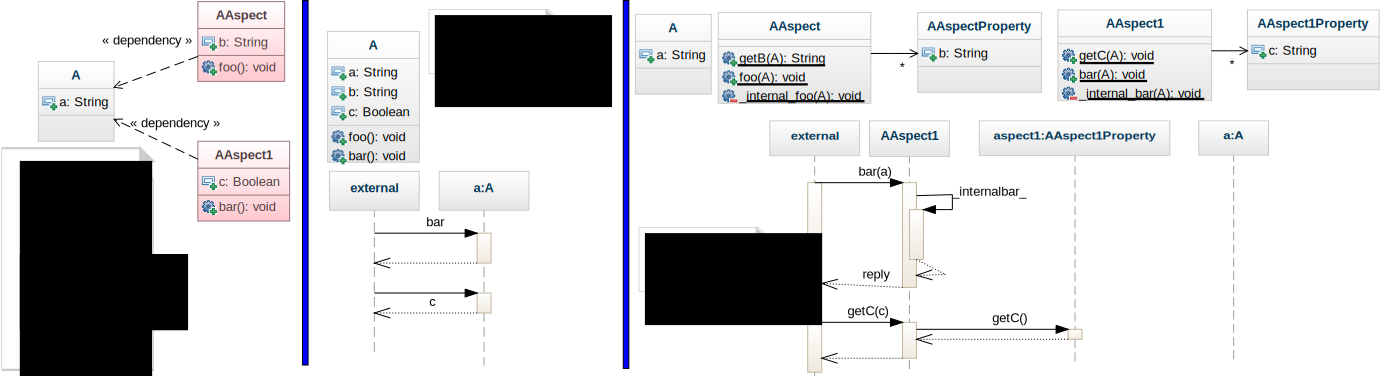
\includegraphics[width=0.9\linewidth]{chapter2/fig/famous}
\caption{Translation process used for building developer abstraction using annotations}
\label{fig:k3-diagram}
\end{figure*}

\section{Component-oriented Resource Awareness} \label{sec:components-oriented-resource-awareness}

Developing applications by reusing independent units of software is the field of study of the Component-Based Software Engineer's community (CBSE community) \cite{cbse-conference}.
By providing a common understanding of component, connector and configuration, CBSE aims at reducing complexity in software development and maintenance \cite{xadl,Medvidovic:2000,VanOmmering-et-al-00}.
%CBSE aims at reducing complexity through abstraction and separation of concerns by providing a common understanding of component, connector and configuration~\cite{xadl,Medvidovic:2000,VanOmmering-et-al-00}.
In addition to economical benefits such as reducing time to market and development cost \cite{SZYPERSKI2002}, there are also technical advantages in using CBSE. 
One of this benefits is that it facilitates the management of dynamic architectures, which becomes, for instance, a primary concern in the Future Internet and Cyber-Physical Systems~\cite{DBLP:journals/ase/NittoGMPP08, Johnson:2015:CSM:2735960.2735979}.
Such systems demand techniques that let software react to changes by self-organizing its structure and self-adapting its behavior~\cite{PanzicaLaManna:2012:LDU:2304736.2304764, Johnson:2015:CSM:2735960.2735979, Zhang:2009:MVD:1509239.1509262}.
Many works~\cite{cbse-conference} have shown the benefits of using component-based approaches in such open-world environments~\cite{baresi2006toward, Caporuscio:2010:AIA:1985522.1985547, Perez-Palacin:2010:PAO:1712605.1712614}.

In a general sense, the concept that embodies the idea behind software components can be defined as follow
\cite{Crnkovic2011}:

\begin{description}
\item[Definition 1:] A \textit{Software Component} is a software building block that conforms to a component model. 
\item[Definition 2:] A \textit{Component Model} defines standards for (i) properties that individual components must satisfy; and (ii) methods, and possibly mechanisms, for composing components.
\end{description}

Despite of the existence of many research and practitioner approaches to component-based programming have been developed \cite{Heineman2001, SZYPERSKI2002, Crnkovic2011}, this broad definition is able to successfully spot the commonalities of a plethora of different component models.
However, plenty of diversity exists in current component models and frameworks.
They tend to target different technologies, aim at different use cases, provide support for different concerns, and use different design principles.

In practice, a framework to compare and classify component models, as the one presented by Crnkovic et al.
\cite{Crnkovic2011}, results useful.
It allows us to focus on those properties that characterize component models.
The aforementioned classification framework proposes three dimensions that are of interest to us: \textit{life-cycle}, \textit{constructs}, and \textit{support for extra-functional properties (EFP)}.
A brief description of these dimensions is given below:

\paragraph{Life-cycle:}

This dimension embodies properties such as \textit{modeling capabilities}, which describe component model's support for the modeling and the design of component-based systems and components; 
\textit{implementation support}, which basically describes the language that can be used to develop components; and \textit{deployment capabilities}, which describe whether components can be deployed at runtime.

In this thesis, we are interested in component models that provide \textit{modeling capabilities} during the development phase.
However, we also require minimal support for querying a system architecture at runtime. 
In addition, we are only interested in component models that target MRTEs, such as Java and .Net.
Finally, to satisfy the needs for adaptation, several component models provide solutions to dynamically reconfigure a software architecture through, for example, the deployment of new modules, the instantiation of new services, and the creation of new bindings between components~\cite{Porter:2014:RMC:2602458.2602471, Zheng:2014:RCC:2679601.2680405, Irmert:2008:RAS:1370018.1370036, Ghezzi:2010:QDD:2163764.2163774}. 
In practice, component-based (and/or service-based) platforms like Fractal~\cite{bruneton06}, OpenCOM~\cite{BlairCULJ04}, OSGi~\cite{OSGI:r5} or SCA~\cite{SEINTURIER:2011:INRIA-00567442:1} provide platform mechanisms to support dynamic architectures; this requires the capability of deploying components at runtime.
Since, we are dealing with the problem of supporting resource awareness in open environments, we focus on those component models that allow component deployment at runtime.


\paragraph{Constructs:}

A set of properties that mainly describe how components communicate are included in this dimension;
some of these properties are: the \textit{existence of ports}; if there exists distinction between \textit{required/provided interfaces}; \textit{interface language}, which the language used to describe interfaces; the \textit{interface levels}, which are limited in such a framework to syntactic, semantic, and behavior; and the \textit{communication type}, which may include synchronous, unicast, and others.
Our interest on this dimension is limited to understand what mechanisms are used to support interaction between components, how are these mechanisms implemented, and how interaction between components affects the way in which we deal with resource consumption monitoring and reservation. 

\paragraph{Support for EFPs:}

Support for dealing with EFPs has not been standardized among component models.
This is a consequence of facts such as the diversity of extra-functional requirements among applications, and the existence of a huge number of properties.
In this dimension, we find the following properties of component models: \textit{EFPs support}, which states whether the component model provides general support for specification and reasoning about EFPs; 
\textit{EFPs specification}, which describes which type of support and/or which properties;
and \textit{Composability of EFPs}, which embodies what properties can be composed and what type of composition is allowed.
In the next section we further describes this dimension in the special case of extra-functional properties that refer to computational resource usage.

\subsection{Extra-functional Properties} \label{sec:efp-resources}

According to \cite{Beugnard774917}, contracts can be classified in four levels which, if
taken together, form a global contract; these are syntactic level, behavioral level, synchronization level, and Quality-Of-Service level.
Contracts based on the first three levels describe what can be done under which provisions.
They do not specify other properties such as how long it would take to service a request or what other resources, besides time, would be consumed by a component in order to perform some action.
Nevertheless, in real scenarios, a violation of extra-functional
requirements can break clients just as easily as a violation of, for instance, a business rule. 
If a provider is too slow in performing a function, any client component will also be slow in achieving their goal.
Without using contract on QoS to control performance, it can be hard to identify what components are underperforming. 
Beside time, components have to respect other resource limitations such as excessive heap storage and network usage.

\paragraph{Where are the mechanism for managing EFPs implemented?}
Two interesting aspects of EFPs management are i) selecting which actors implement the mechanism and policies to manage extra-functional aspects, and ii) deciding if the actors will collaborate to achieve EFPs management \cite{Crnkovic2011}.

Many component models provide no facilities for managing EFPs.
The mechanism used to handle a property is left to the designers of each application; as a result, a
property may not be managed at all.
This solution facilitates the creation of EFP management policies that are specifically tuned towards a system, and also supports the usage of multiple policies in a system.
However, the fact that such policies are not
standardized (and are fully implemented in components) may be a source of architectural mismatch between
components.

The compatibility of components is improved if the
component model provides standardized facilities for managing EFPs.
In this approach, the component execution platform contains
policies for managing EFPs for individual components as well as for EFPs involving multiple components.
The ability to negotiate the manner in which EFPs are handled requires that the
components themselves have some knowledge about how the EFP affects their functioning.

In yet another approach, components are designed to address only functional aspects and not EFPs.
Thus, in the execution environment, these components
are wrapped in a container that has the knowledge on how to manage EFPs.
Containers can either be totally in charge of managing EFPs or
they can interact with a mechanism in the component framework that manages EFPs.
This approach is a way of realizing separation of
concerns in which components focus on functional aspects
and containers concentrate on extra-functional aspects.
In this way, components are more easy to integrate into multiple systems that employ different policies for EFPs.
Since these components do not tackle EFPs management, another advantage is that they are simpler to implement.

\paragraph{How to account for resource consumption in the presence of interaction between components?}
In the case of extra-functional properties that refer to resource consumption, there are special considerations.
One of the most interesting is how to account for resource consumption when usually components are organized as clients and providers.
This corresponds to the already mentioned concept of resource container \cite{Banga:1999:RCN:296806.296810}.
Two ways to accounting are identified in \cite{Miettinen2008,Maurel:2012:AME:2304736.2304763}:

\begin{description}
\item[direct accounting:] the resources consumed during
components' interaction are accounted to the provider.
For instance, the CPU used by a code that belongs
to component A will be accounted to A, no matter if it the code is being executed on behalf of other components.

\item[indirect accounting:] all the resources consumed to service a request that was originated in a component A are accounted to A.
In other words, there is no resource consumption accounted to service providers.
\end{description}

Both ways have advantages and disadvantages.
For instance, in the case of direct accounting, if a provider is
called in an endless loop, the resource usage will be accounted
to the provider instead of to the client that executes such a loop.
Likewise, if the service is poorly implemented, in indirect accounting the user of the service is identified as the responsible.

\paragraph{How to model contracts regarding resource requirements?}
\todo{Write this}

%\cite{Jung:2011:LAI:2000292.2000296}
%
%Architecting Fault-tolerant Component-based Systems: from requirements to testing
%
%A New Component Concept for Fault Trees
%
%Fault-Tolerance for Component-Based Systems - An Automated Middleware Specialization Approach
%
%otra cosa
%\cite{SZYPERSKI2002,Lau:2014:SCM:2602458.2611456}

\subsection{Component Models}

In the next section, we provide a very brief overview of some component models and their main characteristics.
The discussion is limited to component models that have been either designed from scratch or implemented to target MRTEs.
Since we are interested in software systems that evolve at runtime, the discussion is also limited to component models that allow component deployment at runtime.
The list is not exhaustive; instead, it should be understood as a provision of some characteristic examples.
Nevertheless, a component model - Kevoree -  is discussed in further details because the contributions in chapters \ref{chp:scapegoat} and \ref{chp:squirrel}
are implemented and evaluated using such a component model.

\paragraph{Enterprise Java Beans (EJB)} \cite{OracleEJB3.0} envisions the construction of object-oriented and
distributed business applications in trying to hide to developers the underlying complexity of common operations such as transactions processing, persistence,
concurrency, and interoperability.
It also aims at the improvement of component reusability in providing the so called EJB-jars to package components.
An EJB container holds two major types of components to match the needs of different applications: SessionBean, and MessageDrivenBeans.
Each of these beans is deployed in an EJB Container which is in charge of their management at
runtime (start, stop, activation or deactivation).
Starting with EJB 3.0, annotations are heavily used for dependency injection to simplify configuration and integration of heterogeneous systems. 
In order to achieve this, EJB technology use the Java programming language.

\paragraph{The Open Services Gateway Initiative (OSGi)} \cite{OSGI:r5} is a consortium of industrial partners working together to
define a service-oriented framework with ``open specifications
for the delivery of multiple services over wide area networks to local networks and devices''.
In the OSGi's component definitions, there is a clear distinction between a unit of
composition and a unit of deployment; the former is known as service while the latter is called bundle.
OSGi offers a flexible architecture of systems that can dynamically evolve during execution time.
This implies that in the system, components can be added, removed or modified at run-time.
Thus, there is no guaranty that a service provided at a certain time will be still provided later.
Being built on Java, on which it heavily depends, OSGI is platform independent.

%\paragraph{Fractal} \cite{Bruneton:2006:FCM:1152333.1152345} is a hierarchical and reflective component model with sharing.
%Components in this model can be endowed with arbitrary reflective capabilities, from plain black-box objects to
%components that allow a fine-grained manipulation of their internal structure.
%The paper describes JULIA, a Java implementation of the model, a small but efficient runtime framework, which relies on
%a combination of interceptors and mixins for the programming of reflective features of components.
%The paper presents a qualitative and quantitative evaluation of this implementation, showing that
%component-based programming in FRACTAL can be made very efficient. 

\paragraph{Fractal} \cite{Bruneton:2006:FCM:1152333.1152345} intends to cover the whole development lifecycle (design, implementation, deployment and maintenance/management) of complex systems.
It comes up with features such as nesting, sharing of components and reflexivity.
In other words, a component may respectively be created from other components, be shared between components and describes its own behavior.
Fractal aims at providing an general model that can be tuned to fit a large variety of applications and domains.
Hence, nothing is fixed in Fractal.
Actually, since the component model is language and platform independent, it is possible to leverage domain-specific 
For instance, there exists a C-implementation called Think \cite{Fassino:2002:TSF:647057.713860}, 
a Java-implementation called Julia \cite{Bruneton:2006:FCM:1152333.1152345}.
Fractal can be seen as a generic component model which intends to encompass other component models.

\paragraph{SOFA 2.0 (Software Appliances)} components are specified by their frame and architecture \cite{Bures2006}.
A frame can be considered a black box that defines the provided and required interfaces, and its properties.
However, a frame can also be a composite component where the structure of a component is described until the first level of nesting in the component hierarchy.
In SOFA, components and systems are defined using a ADL language: Component Description Language (CDL).
The resulting CDL is compiled to create a system implementation in a programming
language such as C++ or Java.
%SOFA components can be composed by method calls through connectors.
The SOFA 2.0 component model add support for new services: dynamic reconfiguration, control interfaces and multiple communication styles between the components.

\paragraph{Palladio}

\paragraph{Kevoree}
Built on top of dynamic component frameworks, Models@run.time denote model-driven approaches that aim at taming the complexity of dynamic adaptation.
It basically pushes the idea of reflection~\cite{morin09a} one step further by considering the reflection-layer as a real model: ``something simpler, safer or cheaper than reality to avoid the complexity, danger and irreversibility of reality''.
In practice, component-based and service-based platforms offer reflection APIs that allow instrospecting the application (e.g., which components and bindings are currently in place in the system) and dynamic adaptation (e.g., changing the current components and bindings).
While some of these platforms offer rollback mechanisms to recover after an erroneous adaptation~\cite{leger2010reliable}, the purpose of Models@run.time is to prevent the system from actually enacting an erroneous adaptation. 
In other words, the ``model at runtime'' is a reflection model that can be decoupled from the application (for reasoning, validation, and simulation purposes) and then automatically resynchronized.
This model can not only manage the application's structural information (i.e., the architecture), but can also be populated with behavioural information from the specification or the runtime monitoring data.

Kevoree provides multiple concepts that are used to create a distributed application that allows dynamic adaptation. The \emph{Node} concept is used to model the infrastructure topology and the \emph{Group} concept is used to model the semantics of inter-node communication, particularly when synchronizing the reflection model among nodes. 
Kevoree includes a \emph{Channel} concept to allow for different communication semantics between remote \emph{Components} deployed on heterogeneous nodes. 
All Kevoree concepts (\textit{Component}, \textit{Channel}, \textit{Node}, \textit{Group}) obey the object type design pattern~\cite{johnson_type_1997} in order to separate deployment artifacts from running artifacts.  

%Platforms
Kevoree supports multiple execution platforms (e.g.,~Java, Android, MiniCloud, FreeBSD, Arduino). For each target platform it provides a specific runtime container. 
%Tools
Moreover, Kevoree comes with a set of tools for building dynamic applications (a graphical editor to visualize and edit configurations, a textual language to express reconfigurations, several checkers to valid configurations). 

As a result, Kevoree provides a promising environment by facilitating the implementation of dynamically reconfigurable applications in the context of an open-world environment.
Because our goal is to design and implement an adaptive monitoring system, the introspection and the dynamic reconfiguration facilities offered by Kevoree suit the needs of the ScapeGoat framework.

\todo{READ UNTIL THIS POINT}

\section{State of the art of resource management for components} \label{sec:component-leverage}
\begin{itemize}
\item Describe las soluciones de kouther
\item generacion de contenedores
\item generacion de canales de comunicacion
\item ver que mas se puede describir
\end{itemize}


Franz Brosch, Heiko Koziolek, Barbora Buhnova, Ralf Reussner: Architecture-Based Reliability Prediction with the Palladio Component Model. IEEE Trans. Software Eng. 38(6): 1319-1339 (2012)

Sam Malek, Marija Mikic-Rakic, Nenad Medvidovic: A Style-Aware Architectural Middleware for Resource-Constrained, Distributed Systems. IEEE Trans. Software Eng. 31(3): 256-272 (2005)

Anne Koziolek, Ralf Reussner: Towards a generic quality optimisation framework for component-based system models. CBSE 2011: 103-108

Marco Autili, Paolo Di Benedetto, Paola Inverardi: Context-Aware Adaptive Services: The PLASTIC Approach. FASE 2009: 124-139

Mauro Caporuscio, Antinisca Di Marco, Paola Inverardi: Model-based system reconfiguration for dynamic performance management. Journal of Systems and Software 80(4): 455-473 (2007)

Marco Autili, Paolo Di Benedetto and Paola Inverardi, Hybrid Approach for Resource-based Comparison of Adaptable Java Applications (2012), in: Journal of Science of Computer Programming (SCP)

\section{Domain-Specific Languages and MRTEs} \label{sec:DSL-on-MRTEs}

In software engineer, models are abstractions of a software system and its environment.
Model-Driven Software Development (MDSD) puts analysis and design models on par with
code because their implementation is automated~\cite{Stahl:2006:MSD:1196766, Fowler:2010:DSL:1809745}.
The usefulness of a model is limited to the domain it represents.
In other words, a model may be useful for answering a class of questions, but it may fail in answering other questions.
MDSD aims to describe domain-specific abstractions and makes them accessible through formal modeling.
A set of abstractions and their relationships is called, in the context of MDSD, a Metamodel or Domain-Specific Language (DSL)~\cite{Fowler:2010:DSL:1809745}.
Typically, models are translated to source code written in some general purposes language to enable their subsequent compilation and execution.
However, models are also useful in other tasks such as generating test cases \cite{Kiffe2009,Gutierrez2015}, simulating a system behavior \cite{Broenink2012,brosig2015a,Bocciarelli2015425}, and formally verifying software properties \cite{Holzmann2004,Henriksson2005101,Moffett2013,DiGuglielmo20132013}. 

DSLs can be roughly classified as internal or external DSLs.
An internal DSL is embedded into a general-purpose language.
Often, meta-programming facilities, of either a dynamically typed host language or a statically typed language with type inference, are used to seamless integrate the DSL into the host language.
On the contrary, a ``\textit{program}'' written using an external DSL requires a separated translation process (i.e., compilation) in order to produce an artifact that can be integrated as part of an application.
Both approaches have advantages and disadvantages.
Internal DSLs can leverage all the features of their host languages, and it is easy to use constructor of the DSL as extensions of the host language.
However, the concrete syntax of an internal DSL most be carefully crafted to cope with the constrains in the host language's syntax.
On the contrary, there is complete freedom in deciding the concrete syntax of external DSLs; as a designer you can even choose not to use a textual syntax.
Another interesting point is that Integrated Development Environment (IDE) support for internal DSLs is limited to the support provided to the host language.


MDSD consists of two major aspects: processing models and creating models.
The creation of models can be achieved with graphical~\cite{Kolovos:2009:RLA:1564600.1564699, Biermann:2006:GDI:2087202.2087244} or textual editors~\cite{Merkle:2010:TMT:1869542.1869564}.
A well known framework for building DSLs is Xtext~\cite{Eysholdt:2010:XIY:1869542.1869625}.
It is an Eclipse-based framework which supports the definition of languages together with their syntaxes, semantic checkers, code generators and even code editors.

\section{Resource Awareness for Domain-specific Abstractions} \label{sec:resource-awareness-for-dsl}

\subsection{Languages to deal with resource aware}

\paragraph{DiSL: a domain-specific language for bytecode instrumentation, \cite{Marek:2012:DEL:2162037.2162046,Marek2012}}
Dynamic program analysis tools support numerous software engineering tasks, including profiling, debugging, and re-
verse engineering.
Prevailing techniques for building dynamic analysis tools are based on low-level abstractions
that make tool development tedious, error-prone, and expensive. To simplify the development of dynamic analysis tools,
some researchers promoted the use of aspect-oriented programming (AOP). However, as mainstream AOP languages
have not been designed to meet the requirements of dynamic analysis, the success of using AOP in this context remains
limited. For example, in AspectJ, join points that are important for dynamic program analysis (e.g., the execution of
bytecodes or basic blocks of code) are missing, access to reflective dynamic join point information is expensive, data
passing between woven advice in local variables is not supported, and the mixing of low-level bytecode instrumentation
and high-level AOP code is not foreseen. In this talk, we present DiSL [1], a new domain-specific aspect language for
bytecode instrumentation.
DiSL uses Java annotation syntax such that standard Java compilers can be used for compiling
DiSL code. The language features an open join point model, novel constructs inspired by weave-time evaluation of
conditional join points and by staged execution, and access to custom static and dynamic context information.
Moreover, the DiSL weaver guarantees complete bytecode coverage.
We have implemented several dynamic analysis tools in DiSL,
including profilers for the inter- and intra-procedural control
flow, debuggers, dynamic metrics collectors integrated in the
Eclipse IDE to augment the static source views with dynamic information, and tools for workload characterization.
These tools are concise and perform equally well as implementations using low-level techniques. DiSL has also been
conceived as an intermediate language for future domain-specific analysis languages, as well as for AOP languages.

\paragraph{Javana: A System for Building Customized Java Program Analysis Tools, \cite{Maebe06javana:a}}
Understanding the behavior of applications running on high-level
language virtual machines, as is the case in Java, is non-trivial because of the tight entanglement at the lowest execution level between the application and the virtual machine.

This paper proposes Javana, a system for building Java program analysis tools.
Javana provides an easy-to-use instrumentation infrastructure that allows
for building customized profiling tools very quickly.
Javana runs a dynamic binary instrumentation tool underneath
the virtual machine. The virtual machine communicates with the
instrumentation layer through an event handling mechanism for
building a vertical map that links low-level native instruction pointers and memory addresses to high-level language concepts such as
objects, methods, threads, lines of code, etc.
The dynamic binary instrumentation tool then intercepts all memory accesses and instructions executed and provides the Javana end user with high-
level language information for all memory accesses and natively
executed instructions.

We demonstrate the power of Javana through a number of applications: memory address tracing, vertical cache simulation and
object lifetime computation.
For each of these applications, the instrumentation specification requires only a small number of lines
of code.
Developing similarly powerful profiling tools within a virtual machine (as done in current practice) is both time-consuming
and error-prone; in addition, the accuracy of the obtained profiling
results might be questionable as we show in this paper.
\paragraph{Flexible and efficient profiling with aspect-oriented programming, \cite{Binder:2006:FEM:1173706.1173733}}
Many profilers for virtual execution environments, such as the Java virtual machine (JVM), are implemented with low-level bytecode instrumentation techniques, which is tedious, error-prone, and complicates maintenance and extension of the tools.
In order to reduce the development time and cost, we promote building profilers for the JVM using high-level aspect-oriented programming (AOP).
We show that the use of aspects yields concise profilers that are easy to develop, extend, and maintain, because low-level
instrumentation details are hidden from the tool developer.
In order to build efficient profilers, we introduce inter-advice communication, an extension to common AOP languages that enables efficient data passing
between advices that are woven into the same method using local variables.
We illustrate our approach with two case studies.
First, we show that an existing, instrumentation-based tool for listener latency
profiling can be easily recast as an aspect.
Second, we present an aspect for comprehensive calling context profiling.
In order to reduce profiling overhead, our aspect parallelizes application execution and profile
creation, resulting in a speedup of 110\% on a machine with more than two cores, compared with a primitive, non-parallel approach
\paragraph{A portable and customizable profiling framework for Java based on bytecode instruction counting, \cite{Binder2005}}
Prevailing profilers for Java, which rely on standard, native-code profiling interfaces, are not portable, give imprecise results due to serious measurement perturbation, and cause excessive overheads.
In contrast, program transformations allow to generate reproducible profiles in a fully portable way with significantly less overhead.
This paper presents a profiling framework that instruments Java programs at the bytecode level to build context-sensitive execution profiles at runtime.
The profiling framework includes an exact profiler as well as a sampling profiler.
User-defined profiling agents can be written in pure Java, too, in order to customize the runtime processing of profiling data.
\paragraph{Profiling with AspectJ, \cite{Pearce:2007:PA:1248445.1248448}}
This paper investigates whether AspectJ can be used for efficient profiling of Java programs.
Profiling differs from other applications of AOP (e.g. tracing), since it necessitates efficient and often complex
interactions with the target program.
As such, it was uncertain whether AspectJ could achieve this goal.
Therefore, we investigate four common profiling problems (heap usage, object lifetime, wasted time and
time-spent) and report on how well AspectJ handles them.
For each, we provide an efficient implementation,
discuss any trade-offs or limitations and present the results of an experimental evaluation into the costs
of using it.
Our conclusions are mixed. On the one hand, we find that AspectJ is sufficiently expressive
to describe the four profiling problems and reasonably efficient in most cases.
On the other hand, we find several limitations with the current AspectJ implementation that severely hamper its suitability for
profiling.

\paragraph{Controlled dynamic performance analysis, \cite{Reiss:2008:CDP:1383559.1383566}}
We are interested in obtaining detailed performance information
on-the-fly from long-running systems without adversely affecting
the performance of the systems.
We have developed a methodology consisting of a framework, DYPER, and a number of
specialized agents called proflets each of which analyzes a
different performance aspect.
DYPER gathers performance information with a guaranteed maximum overhead that is
dynamically settable by the programmer using priorities set by the
proflets.
Moreover, the type of information that the system can
provide is generally only available for tools that generally have too
much overhead to be usable in production or long-running
systems.
DYPER includes the ability to control and display
performance data as the program is run.

\paragraph{A meta-aspect protocol for developing dynamic analyses, \cite{Achenbach:2010:MPD:1939399.1939415} }
Dynamic aspect-oriented programming has been widely used
for the development of dynamic analyses to abstract over low-level program instrumentation.
Due to particular feature requirements in different analysis domains like debugging or testing, many different aspect
languages were developed from scratch or by extensive compiler or interpreter extensions.
We introduce another level of abstraction in form of a meta-aspect protocol to separate the host language from the analysis
domain.
A language expert can use this protocol to tailor an analysis-specific aspect language, based on which a domain expert can develop
a particular analysis.
Our design enables a flexible specification of the join point model, configurability of aspect deployment and scoping, and
extensibility of pointcut and advice language.
We present the application of our design to different dynamic analysis domains.
\paragraph{Comprehensive Profiling Support in the Java Virtual Machine. \cite{Liang1999}}
Existing profilers for Java applications typically rely on custom instrumentation in the Java virtual machine, and measure only limited types of resource consumption. Garbage collection and multi-threading pose additional challenges to profiler design and implementation.

In this paper we discuss a general-purpose, portable, and extensible approach for obtaining comprehensive profiling information from the Java virtual machine. Profilers based on this framework can uncover CPU usage hot spots, heavy memory allocation sites, unnecessary object retention, contended monitors, and thread deadlocks. In addition, we discuss a novel algorithm for thread-aware statistical CPU time profiling, a heap profiling technique independent of the garbage collection implementation, and support for interactive profiling with minimum overhead. 
\paragraph{Profiling Field Initialisation in Java, \cite{Nelson2013}}
\todo{No cre que sea muy bueno}
Java encourages programmers to use constructor methods to
initialise objects, supports final modifiers for documenting fields which
are never modified and employs static checking to ensure such fields
are only ever initialised inside constructors. Unkel and Lam observed
that relatively few fields are actually declared final and showed using
static analysis that many more fields have final behaviour, and even more
fields are stationary (i.e. all writes occur before all reads). We present
results from a runtime analysis of 14 real-world Java programs which
not only replicates Unkel and Lam’s results, but suggests their analysis
may have under-approximated the true figure. Our results indicate a
remarkable 72-82% of fields are stationary, that final is poorly utilised by
Java programmers, and that initialisation of immutable fields frequently
occurs after constructor return. This suggests that the final modifier for
fields does a poor job of supporting common programming practices.
\paragraph{A dynamic optimization framework for a Java just-in-time compiler, \cite{Suganuma:2001:DOF:504311.504296}}
The high performance implementation of Java Virtual Machines (JVM) and just-in-time (JIT) compilers is directed toward adaptive compilation optimizations on the basis of online runtime profile information. This paper describes the design and implementation of a dynamic optimization framework in a production-level Java JIT compiler. Our approach is to employ a mixed mode interpreter and a three level optimizing compiler, supporting quick, full, and special optimization, each of which has a different set of tradeoffs between compilation overhead and execution speed. a lightweight sampling profiler operates continuously during the entire program's exectuion. When necessary, detailed information on runtime behavior is collected by dynmiacally generating instrumentation code which can be installed to and uninstalled from the specified recompilation target code. Value profiling with this instrumentation mechanism allows fully automatic code specialization to be performed on the basis of specific parameter values or global data at the highest optimization level. The experimental results show that our approach offers high performance and a low code expansion ratio in both program startup and steady state measurements in comparison to the compile-only approach, and that the code specialization can also contribute modest performance improvement.

\paragraph{Complete and Platform-Independent Calling Context Profiling for the Java Virtual Machine, \cite{Sarimbekov201161}}
Calling context profiling collects statistics separately for each calling context. Complete calling context profiles that faithfully represent overall program execution are important for a sound analysis of program behavior, which in turn is important for program understanding, reverse engineering, and workload characterization. Many existing calling context profilers for Java rely on sampling or on incomplete instrumentation techniques, yielding incomplete profiles; others rely on Java Virtual Machine (JVM) modifications or work only with one specific JVM, thus compromising portability. In this paper we present a new calling context profiler for Java that reconciles completeness of the collected profiles and full compatibility with any standard JVM. In order to reduce measurement perturbation, our profiler collects platform-independent dynamic metrics, such as the number of method invocations and the number of executed bytecodes. In contrast to prevailing calling context profilers, our tool is able to distinguish between multiple call sites in a method and supports selective profiling of (the dynamic extent of) certain methods. We have evaluate the overhead introduced by our profiler with standard Java and Scala benchmarks on a range of different JVMs.

\subsection{Query languages about memory management}

In DeAl~\cite{Reichenbach:2010:GCE:1869459.1869482}, the authors propose a language to compute heap assertions at garbage collection time.
The language design is motivated by concerns of efficiency as our approach.
There is however a large number of differences, first DeAl is only able to compute boolean outputs while our DSL is intended to produce arbitrary data type as output which also includes boolean values.
DeAl is a purely declarative language while our DSL contains a much more complex execution model.
In exchange for the declarative style and the focus on assertions, DeAl is able to guarantee formal properties about the computation that we cannot provide. 

In~\cite{Xu:2013:PML:2491509.2491511} the authors propose a framework to detect memory leaks associated with Java containers.
To do so, the framework explores the status of each container object with the goal of identifying leak patterns. The approach is based on finding objects which are keeping references to removed bundles. LeakBots~\cite{Mitchell03leakbot:an} is an automated tool to detect memory leaks. It makes heavy
use of information recollected from the heap in order to identify the more likely structures leading to a leak.
These tools collect data from the heap in order to automatically pinpoint a particular memory issue.
The methods to collect the data are handwritten for efficiency reasons.
Lots of data collected in these works is also available with our approach.

\paragraph{another, \cite{Harkema:2002:PMJ:584369.584388}}

\subsection{Debugging support for DSLs}

\section{Conclusions}

Discutir aqui que problemas nuevos surgen cuando se quiere hacer resource management en component-based systems. Por ejemplo, a quien se le asigna el consumo.


